\documentclass[letter,11pt]{article}

\usepackage[spanish,es-nodecimaldot]{babel}
\usepackage[utf8]{inputenc}

\usepackage{lmodern}
\usepackage[T1]{fontenc}
\usepackage{textcomp}

\usepackage{framed}
\usepackage[svgnames]{xcolor}
\colorlet{shadecolor}{Gainsboro!50}

\usepackage[labelfont=bf]{caption}
\usepackage{graphicx}
\usepackage{pstricks}

\usepackage{anysize}
\marginsize{3cm}{2cm}{2cm}{3cm}

\usepackage{siunitx}
\usepackage{amsmath}
\usepackage{array}
\usepackage{csquotes}
\usepackage{steinmetz}

\usepackage{fancyhdr}
\usepackage{lastpage}
\pagestyle{fancy}
\fancyhf{}
\fancyhead[LE,RO]{Laboratorio de Circuitos Eléctricos III}
\fancyfoot[CO,CE]{\thepage\ de \pageref{LastPage}}

\special{papersize=215.9mm,279.4mm}

\usepackage[
    pdfauthor={Carlos Eduardo Caballero Burgoa},%
    pdftitle={Laboratorio de Circuitos Eléctricos III},%
    pdfsubject={Circuitos trifásicos desequilibrados con fuente estrella y carga estrella},%
    colorlinks,%
    citecolor=black,%
    filecolor=black,%
    linkcolor=black,%
    urlcolor=black,
    breaklinks]{hyperref}
\usepackage{breakurl}

\renewcommand{\arraystretch}{1.2}

\begin{document}

\begin{titlepage}
    \begin{center}
        {\Large UNIVERSIDAD MAYOR DE SAN SIMÓN}\\
        \vspace*{0.15cm}
        {\large FACULTAD DE CIENCIAS Y TECNOLOGÍA}\\
        \vspace*{0.10cm}
        DEPARTAMENTO DE ELÉCTRICA-ELECTRÓNICA\\
        \vspace*{3.0cm}
        {\Large \textbf{LABORATORIO DE CIRCUITOS ELÉCTRICOS III}}\\
        \vspace*{0.3cm}
        {\Large \textbf{INFORME No. 3}}\\
        \vspace*{3.5cm}
        {\Large \textbf{CIRCUITOS TRIFÁSICOS DESEQUILIBRADOS \\
        CON FUENTE ESTRELLA Y CARGA ESTRELLA}}\\
    \end{center}

    \vspace*{5.8cm}
    \leftskip=7.95cm
    \noindent
    \textbf{Estudiante:}\\
    Caballero Burgoa, Carlos Eduardo.\\
    \newline
    \textbf{Carrera:}\\
    Ing. Electromecánica.\\
    \newline
    \textbf{Docente:}\\
    Ing. Marco Antonio Vallejo Camacho.\\
    \newline
    \textbf{Grupo:} 2F (Martes).\\
\textbf{Fecha de entrega:} 1 de Octubre del 2024.\\
\end{titlepage}

\section{Cálculos teóricos}
Considerando un circuito trifásico estrella-estrella desequilibrado con las
siguientes cargas:

\begin{itemize}
    \item \textbf{Carga A}: $R_1=1[k\Omega]$.
    \item \textbf{Carga B}: $R_2=250[\Omega]$ y $L=1[H]$.
    \item \textbf{Carga C}: $R_3=500[\Omega]$ y $C=10[\mu F]$.
\end{itemize}

Con voltaje de fase $U_L=220[\text{V}]$ y con frecuencia de $50[\text{Hz}]$,
se hallan las corrientes de linea para los siguientes casos:
\\

\subsection{Sin linea de neutro}
\begin{figure}[!h]
\centering
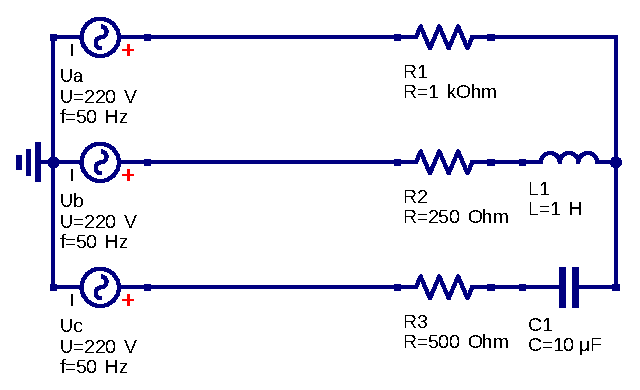
\includegraphics[scale=0.9]{figura1.eps}
\caption{Circuito trifásico desequilibrado sin linea de neutro.}
\label{circuito1}
\end{figure}

\subsubsection{Secuencia positiva}
Se calcula la frecuencia angular ($\omega$):
\begin{equation*}
    \begin{split}
        \omega&=2\pi f\\
              &=2\pi(50)\\
              &=100\pi[\text{rad}/\text{s}]\\
    \end{split}
\end{equation*}

Se hallan las impedancias en el dominio de frecuencia:
\begin{equation*}
    \begin{split}
        Z_1 &= R_1\\
            &= 1000[\Omega]\\
    \end{split}
\end{equation*}

\begin{equation*}
    \begin{split}
        Z_2 &= R_2+j\omega L\\
            &= 250+j100\pi[\Omega]\\
    \end{split}
\end{equation*}

\begin{equation*}
    \begin{split}
        Z_3 &= R_3+\frac{1}{j\omega C}\\
            &= 500-j\frac{1000}{\pi}[\Omega]\\
    \end{split}
\end{equation*}

Considerando una secuencia positiva:
\begin{equation*}
    \begin{split}
        U_a = 220\phase{0^{\circ}}\,[\text{V}]\\
        U_b = 220\phase{-120^{\circ}}\,[\text{V}]\\
        U_c = 220\phase{120^{\circ}}\,[\text{V}]\\
    \end{split}
\end{equation*}

Se calcula el voltaje entre neutros con el teorema de \emph{Millman}:
\begin{equation*}
    \begin{split}
        U_0 &= \dfrac{
                   \dfrac{U_a}{Z_1}+\dfrac{U_b}{Z_2}+\dfrac{U_c}{Z_3}
               }{
                   \dfrac{1}{Z_1}+\dfrac{1}{Z_2}+\dfrac{1}{Z_3}
               }\\
            &= \dfrac{
                   \dfrac{220\phase{0^{\circ}}}{1000}+
                   \dfrac{220\phase{-120^{\circ}}}{250+j100\pi}+
                   \dfrac{120\phase{120^{\circ}}}{500-j(1000/\pi)}
               }{
                   \dfrac{1}{1000}+
                   \dfrac{1}{250+j100\pi}+
                   \dfrac{1}{500-j(1000/\pi)}
               }\\
            &= 159.99\phase{-173.20^{\circ}}[\text{V}]\\
    \end{split}
\end{equation*}

A partir del voltaje de neutro se calculan las corrientes de linea:
\begin{equation*}
    \begin{split}
        I_{L_1} &= \frac{U_a - U_0}{Z_1}\\
                &= \frac{200\phase{0^{\circ}}-159.99\phase{-173.20^{\circ}}}{500}\\
                &= 0.38\phase{2.86^{\circ}}[\text{A}]\\
    \end{split}
\end{equation*}
\begin{equation*}
    \begin{split}
        I_{L_2} &= \frac{U_b - U_0}{Z_2}\\
                &= \frac{200\phase{-120^{\circ}}-159.99\phase{-173.20^{\circ}}}{250+j100\pi}\\
                &= 0.44\phase{-125.59^{\circ}}[\text{A}]\\
    \end{split}
\end{equation*}
\begin{equation*}
    \begin{split}
        I_{L_3} &= \frac{U_c - U_0}{Z_3}\\
                &= \frac{200\phase{120^{\circ}}-159.99\phase{-173.20^{\circ}}}{500-j(1000/\pi)}\\
                &= 0.36\phase{109.35^{\circ}}[\text{A}]\\
    \end{split}
\end{equation*}
\\

\subsubsection{Secuencia negativa}
Considerando una secuencia negativa:
\begin{equation*}
    \begin{split}
        U_a = 220\phase{0^{\circ}}\,[\text{V}]\\
        U_b = 220\phase{120^{\circ}}\,[\text{V}]\\
        U_c = 220\phase{-120^{\circ}}\,[\text{V}]\\
    \end{split}
\end{equation*}

Se calcula el voltaje entre neutros con el teorema de \emph{Millman}:
\begin{equation*}
    \begin{split}
        U_0 &= \dfrac{
                   \dfrac{U_a}{Z_1}+\dfrac{U_b}{Z_2}+\dfrac{U_c}{Z_3}
               }{
                   \dfrac{1}{Z_1}+\dfrac{1}{Z_2}+\dfrac{1}{Z_3}
               }\\
            &= \dfrac{
                   \dfrac{220\phase{0^{\circ}}}{1000}+
                   \dfrac{220\phase{120^{\circ}}}{250+j100\pi}+
                   \dfrac{120\phase{-120^{\circ}}}{500-j(1000/\pi)}
               }{
                   \dfrac{1}{1000}+
                   \dfrac{1}{250+j100\pi}+
                   \dfrac{1}{500-j(1000/\pi)}
               }\\
            &= 111.57\phase{32.36^{\circ}}[\text{V}]\\
    \end{split}
\end{equation*}

A partir del voltaje de neutro se calculan las corrientes de linea:
\begin{equation*}
    \begin{split}
        I_{L_1} &= \frac{U_a - U_0}{Z_1}\\
                &= \frac{200\phase{0^{\circ}}-111.57\phase{32.36^{\circ}}}{500}\\
                &= 0.14\phase{-25.40^{\circ}}[\text{A}]\\
    \end{split}
\end{equation*}
\begin{equation*}
    \begin{split}
        I_{L_2} &= \frac{U_b - U_0}{Z_2}\\
                &= \frac{200\phase{-120^{\circ}}-111.57\phase{32.36^{\circ}}}{250+j100\pi}\\
                &= 0.60\phase{95.87^{\circ}}[\text{A}]\\
    \end{split}
\end{equation*}
\begin{equation*}
    \begin{split}
        I_{L_3} &= \frac{U_c - U_0}{Z_3}\\
                &= \frac{200\phase{120^{\circ}}-111.57\phase{32.36^{\circ}}}{500-j(1000/\pi)}\\
                &= 0.54\phase{-96.74^{\circ}}[\text{A}]\\
    \end{split}
\end{equation*}
\\

\subsection{Con linea de neutro}
\begin{figure}[!h]
\centering
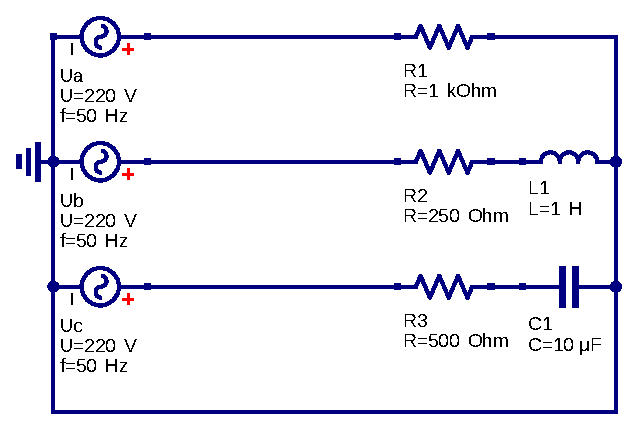
\includegraphics[scale=0.9]{figura2.eps}
\caption{Circuito trifásico desequilibrado con linea de neutro.}
\label{circuito2}
\end{figure}

\subsubsection{Secuencia positiva}
Considerando una secuencia positiva:
\begin{equation*}
    \begin{split}
        U_a = 220\phase{0^{\circ}}\,[\text{V}]\\
        U_b = 220\phase{-120^{\circ}}\,[\text{V}]\\
        U_c = 220\phase{120^{\circ}}\,[\text{V}]\\
    \end{split}
\end{equation*}

Se calculan las corrientes de linea:
\begin{equation*}
    \begin{split}
        I_{L_1} &= \frac{U_a}{Z_1}\\
                &= \frac{200\phase{0^{\circ}}}{500}\\
                &= 0.22\phase{0^{\circ}}[\text{A}]\\
    \end{split}
\end{equation*}
\begin{equation*}
    \begin{split}
        I_{L_2} &= \frac{U_b}{Z_2}\\
                &= \frac{200\phase{-120^{\circ}}}{250+j100\pi}\\
                &= 0.55\phase{-171.49^{\circ}}[\text{A}]\\
    \end{split}
\end{equation*}
\begin{equation*}
    \begin{split}
        I_{L_3} &= \frac{U_c}{Z_3}\\
                &= \frac{200\phase{120^{\circ}}}{500-j(1000/\pi)}\\
                &= 0.37\phase{152.48^{\circ}}[\text{A}]\\
    \end{split}
\end{equation*}

Con las corrientes de linea se calcula la corriente de neutro:
\begin{equation*}
    \begin{split}
        I_0 &= U_{L_1}+U_{L_2}+U_{L_3}\\
            &= 0.22\phase{0^{\circ}}+0.55\phase{-171.49^{\circ}}+0.37\phase{152.48^{\circ}}\\
            &= 0.66\phase{172.10^{\circ}}[\text{A}]\\
    \end{split}
\end{equation*}
\\

\subsubsection{Secuencia negativa}
Considerando una secuencia negativa:
\begin{equation*}
    \begin{split}
        U_a = 220\phase{0^{\circ}}\,[\text{V}]\\
        U_b = 220\phase{120^{\circ}}\,[\text{V}]\\
        U_c = 220\phase{-120^{\circ}}\,[\text{V}]\\
    \end{split}
\end{equation*}

Se calculan las corrientes de linea:
\begin{equation*}
    \begin{split}
        I_{L_1} &= \frac{U_a}{Z_1}\\
                &= \frac{200\phase{0^{\circ}}}{500}\\
                &= 0.22\phase{0^{\circ}}[\text{A}]\\
    \end{split}
\end{equation*}
\begin{equation*}
    \begin{split}
        I_{L_2} &= \frac{U_b}{Z_2}\\
                &= \frac{200\phase{120^{\circ}}}{250+j100\pi}\\
                &= 0.55\phase{68.51^{\circ}}[\text{A}]\\
    \end{split}
\end{equation*}
\begin{equation*}
    \begin{split}
        I_{L_3} &= \frac{U_c}{Z_3}\\
                &= \frac{200\phase{-120^{\circ}}}{500-j(1000/\pi)}\\
                &= 0.37\phase{-87.52^{\circ}}[\text{A}]\\
    \end{split}
\end{equation*}

Con las corrientes de linea se calcula la corriente de neutro:
\begin{equation*}
    \begin{split}
        I_0 &= U_{L_1}+U_{L_2}+U_{L_3}\\
            &= 0.22\phase{0^{\circ}}+0.55\phase{68.51^{\circ}}+0.37\phase{-87.52^{\circ}}\\
            &= 0.46\phase{17.66^{\circ}}[\text{A}]\\
    \end{split}
\end{equation*}
\\

\subsection{Resumen de resultados}
\begin{center}
    \begin{tabular}{|c|c||c|c|c||c|c|}
    \hline
    \multicolumn{2}{|c||}{} &
    $I_{L_1}[\text{A}]$ & $I_{L_2}[\text{A}]$ & $I_{L_3}[\text{A}]$ &
    $U_0[\text{V}]$ & $I_0[\text{A}]$
    \tabularnewline \hline \hline
    $(+)$ & \textbf{SN} &
    $0.38\phase{2.86^{\circ}}$ &
    $0.44\phase{-125.59^{\circ}}$ &
    $0.36\phase{109.35^{\circ}}$ &
    $159.99\phase{-173.20^{\circ}}$ & $-$
    \tabularnewline \hline
    & \textbf{CN} &
    $0.22\phase{0^{\circ}}$ &
    $0.55\phase{-171.49^{\circ}}$ &
    $0.37\phase{152.48^{\circ}}$ &
    $0$ & $0.66\phase{172.10^{\circ}}$
    \tabularnewline \hline
    $(-)$ & \textbf{SN} &
    $0.14\phase{-25.40^{\circ}}$ &
    $0.60\phase{95.87^{\circ}}$ &
    $0.54\phase{-96.74^{\circ}}$ &
    $111.57\phase{32.36^{\circ}}$ & $-$
    \tabularnewline \hline
    & \textbf{CN} &
    $0.22\phase{0^{\circ}}$ &
    $0.55\phase{68.51^{\circ}}$ &
    $0.37\phase{-87.52^{\circ}}$ &
    $0$ & $0.46\phase{17.66^{\circ}}$
    \tabularnewline \hline
    \end{tabular}
\end{center}

\section{Simulación}
Se utilizó el software \emph{Electronic Workbench v5.12.} para simular
los circuitos, estos pueden verse en las figuras: (\ref{simulacion1}),
(\ref{simulacion2}), (\ref{simulacion3}) y (\ref{simulacion4}).

\begin{figure}[!h]
\centering
\includegraphics[scale=0.99]{simulacion/practica3.1.eps}
\caption{Simulación del circuito sin linea de neutro secuencia positiva.}
\label{simulacion1}
\end{figure}

\begin{figure}[!h]
\centering
\includegraphics[scale=0.99]{simulacion/practica3.2.eps}
\caption{Simulación del circuito sin linea de neutro secuencia negativa.}
\label{simulacion2}
\end{figure}

\begin{figure}[!h]
\centering
\includegraphics[scale=0.99]{simulacion/practica3.3.eps}
\caption{Simulación del circuito con linea de neutro secuencia positiva.}
\label{simulacion3}
\end{figure}

\begin{figure}[!h]
\centering
\includegraphics[scale=0.99]{simulacion/practica3.4.eps}
\caption{Simulación del circuito con linea de neutro secuencia negativa.}
\label{simulacion4}
\end{figure}

\section{Tablas y mediciones}
En las tablas siguientes, se presentan los resultados obtenidos con las
mediciones realizadas en laboratorio.

\begin{center}
    \begin{tabular}{|c|c||c|c|c||c|c|c||c|c|}
    \hline
    \multicolumn{2}{|c||}{} &
    $U_{L_1-N}[\text{V}]$ & $U_{L_2-N}[\text{V}]$ & $U_{L_3-N}[\text{V}]$ &
    $I_{L_1}[\text{A}]$ & $I_{L_2}[\text{A}]$ & $I_{L_3}[\text{A}]$ &
    $U_0[\text{V}]$ & $I_0[\text{A}]$
    \tabularnewline \hline \hline
    $(+)$ & \textbf{SN} & $224$ & $222$ & $225$ & $0.36$ & $0.43$ & $0.35$ & $159$ & $-$
    \tabularnewline \hline
          & \textbf{CN} & $225$ & $222$ & $224$ & $0.2$ & $0.53$ & $0.36$ & $0$ & $0.63$
    \tabularnewline \hline
    $(-)$ & \textbf{SN} & $225$ & $222$ & $224$ & $0.12$ & $0.59$ & $0.53$ & $109$ & $-$
    \tabularnewline \hline
          & \textbf{CN} & $225$ & $222$ & $226$ & $0.2$ & $0.53$ & $0.37$ & $0$ & $0.43$
    \tabularnewline \hline
    \end{tabular}
\end{center}

\begin{center}
    \begin{tabular}{|c|c||c|c|c|}
    \hline
    \multicolumn{2}{|c||}{} &
    $U_{Z_1}[\text{V}]$ & $U_{Z_2}[\text{V}]$ & $U_{Z_3}[\text{V}]$
    \tabularnewline \hline \hline
    $(+)$ & \textbf{SN} & $384$ & $184$ & $218$
    \tabularnewline \hline
          & \textbf{CN} & $225$ & $173$ & $225$
    \tabularnewline \hline
    $(-)$ & \textbf{SN} & $146$ & $244$ & $328$
    \tabularnewline \hline
          & \textbf{CN} & $225$ & $222$ & $226$
    \tabularnewline \hline
    \end{tabular}
\end{center}

\section{Cuestionario}

\begin{enumerate}

\item \textbf{¿Existe variación en los valores medidos al cambiar la secuencia
del generador? Qué sucedería en caso de que el sistema fuera equilibrado habría
también variación?. Justifique su respuesta.}

La secuencia del generador determina la fase de los voltajes de fase pero no su
magnitud, como puede verse en las mediciones tomadas.

Las corrientes de fase por otro lado son determinadas mediante la ley de
\emph{Ohm}:

\begin{equation*}
    I_f = \frac{U_f}{Z_Y}
\end{equation*}

Y por tanto, varían según la impedancia conectada en la fase; si las impedancias
conectadas son iguales, las corrientes de fase tendrían la misma magnitud.

\item \textbf{Demostrar el teorema de \emph{Millman} y verifique el valor
calculado con el valor medido en laboratorio. Explique el por qué de las
variaciones si existen.}

Considerando una conexión estrella-estrella:

\begin{figure}[!h]
\centering
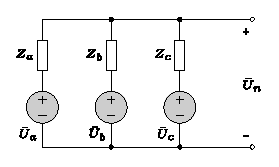
\includegraphics[scale=1.4]{figura3.eps}
\end{figure}

Se calcula el voltaje de neutro por medio del método de voltajes de
nodo:

\begin{equation*}
    \frac{\bar{U}_{n} - \bar{U}_a}{Z_a} + \frac{\bar{U}_{n} - \bar{U}_b}{Z_b} +
    \frac{\bar{U}_{n} - \bar{U}_c}{Z_c} = 0
\end{equation*}
\begin{equation*}
    \frac{\bar{U}_{n}}{Z_a} - \frac{\bar{U}_a}{Z_a} +
    \frac{\bar{U}_{n}}{Z_b} - \frac{\bar{U}_b}{Z_b} +
    \frac{\bar{U}_{n}}{Z_c} - \frac{\bar{U}_c}{Z_c} = 0
\end{equation*}
\begin{equation*}
    \frac{\bar{U}_{n}}{Z_a} + \frac{\bar{U}_{n}}{Z_b} +
    \frac{\bar{U}_{n}}{Z_c} =
    \frac{\bar{U}_a}{Z_a} + \frac{\bar{U}_b}{R_b} +
    \frac{\bar{U}_c}{Z_c}
\end{equation*}
\begin{equation*}
    \bar{U}_{n}\left(\frac{1}{Z_a} + \frac{1}{Z_b} +
    \frac{1}{Z_c} \right) =
    \frac{\bar{U}_a}{Z_a} + \frac{\bar{U}_b}{Z_b} +
    \frac{\bar{U}_c}{Z_c}
\end{equation*}
\begin{equation*}
    \bar{U}_{n}= \dfrac{\dfrac{\bar{U}_a}{Z_a} + \dfrac{\bar{U}_b}{Z_b} +
    \dfrac{\bar{U}_c}{Z_c}}{\dfrac{1}{Z_a} + \dfrac{1}{Z_b} + \dfrac{1}{Z_c}}
\end{equation*}

Los voltajes de neutro a verificar son:
\begin{center}
    \begin{tabular}{|c||c|c|c|}
    \hline
    \textbf{Secuencia} & \textbf{Calculado} & \textbf{Laboratorio} &
    \textbf{Porcentaje de error}
    \tabularnewline \hline \hline
    \textbf{Positiva} & $159.99[V]$ & $159[V]$ & $0.6188\%$
    \tabularnewline \hline
    \textbf{Negativa} & $111.57[V]$ & $109[V]$ & $2.3035\%$
    \tabularnewline \hline
    \end{tabular}
\end{center}

Las variaciones entre el valor calculado y la medición en laboratorio son
mínimas, ocasionadas por la medición.

\item \textbf{Verificar la ley de corrientes de \emph{Kirchhoff} sin neutro
conectado con los valores teóricos calculados, cuánto debería ser y cuánto es lo
que se obtiene?}

En un circuito trifásico estrella-estrella la corriente de linea y la corriente
de fase son iguales, por tanto aplicando la ley de corrientes de
\emph{Kirchhoff} sobre el nodo central de las cargas, se obtiene:

\begin{equation*}
    \begin{split}
        I_{L_1}+I_{L_2}+I_{L_3}=0\\
        0.38\phase{2.86^{\circ}}[\text{A}]+
        0.44\phase{-125.59^{\circ}}[\text{A}]+
        0.36\phase{109.35^{\circ}}[\text{A}]=0\\
        0\phase{11.06}=0\\
    \end{split}
\end{equation*}

El valor es prácticamente $0$.

\item \textbf{Con los datos tomados en el circuito con neutro conectado. ¿El
valor medido de $I_0$ concuerda con lo aprendido en la teoría?}

Las corrientes en la conexión a neutro son:
\begin{center}
    \begin{tabular}{|c||c|c|c|}
    \hline
    \textbf{Secuencia} & \textbf{Calculado} & \textbf{Laboratorio} &
    \textbf{Porcentaje de error}
    \tabularnewline \hline \hline
    \textbf{Positiva} & $0.66[A]$ & $0.63[A]$ & $4.54\%$
    \tabularnewline \hline
    \textbf{Negativa} & $0.46[A]$ & $0.43[A]$ & $6.52\%$
    \tabularnewline \hline
    \end{tabular}
\end{center}

La discrepancia entre el valor calculado y el medido son despreciables.

\item \textbf{Con los datos de laboratorio, ¿existen diferencias de tensiones y
corrientes tanto de fase como de linea, sin neutro y con neutro?. Justifique su
respuesta.}

La variación en los voltajes de fase son mínimos ya sea con conexión a tierra o
sin esta.

La variación en los voltajes de cada impedancia depende de la carga conectada,
que en este caso es diferente para cada conexión.

Respecto a las corrientes de linea/fase estas dependen tanto de la carga
conectada, como del voltaje entre neutros, y también si existe o no conexión
entre ellos, como se describen en las ecuaciones planteadas en la sección de
cálculos.

\end{enumerate}

\section{Conclusiones y Recomendaciones}
Se calcularon, simularon y armaron los diversos circuitos trifásicos, y se pudo
comprobar la variación según la secuencia del generador y la conexión de
neutros para cargas desequilibradas.

Es recomendable al armar los circuitos en laboratorio revisar apropiadamente los
multímetros para la medición de corriente y voltaje, ya que puede ser peligroso
para los equipos cualquier descuido.

\end{document}

